% FAIR'2026 — IEEE conference template (IEEEtran, XeLaTeX, English)
% English translation of the Vietnamese submission (main.tex). Kept in sync.
% Compile: xelatex -> bibtex -> xelatex x2
% Requires: IEEEtran.cls (in ../IEEE-conference-template-062824/), ieeetr.bst.
%
% RESULT PLACEHOLDERS: every empirical number is wrapped in \ph{...}. After
% re-running the (leakage-free) pipeline, replace each \ph{...} with the value
% from the corresponding results/*.csv. Do NOT reuse the legacy F1=1.000
% numbers — they came from a configuration with destination_port leakage and
% feature-level duplicate flows, both now removed.
%
\documentclass[11pt,conference]{IEEEtran}
\usepackage{url}
\IEEEoverridecommandlockouts

\usepackage{fontspec}
\usepackage{polyglossia}
\setdefaultlanguage{english}
\setotherlanguage{vietnamese}
% Shared XeLaTeX font setup for Vietnamese manuscripts.
% TeX Gyre Termes is a Times-compatible font that ships with TeX Live / MacTeX,
% covers Vietnamese, and needs no MS-Office fonts -> builds on any machine.
% If you have "Times New Roman" installed and your venue requires it exactly,
% swap the line below for: \setmainfont{Times New Roman}[Ligatures=TeX]
\setmainfont{TeX Gyre Termes}[Ligatures=TeX]

\usepackage{cite}
\usepackage{graphicx}
\usepackage{booktabs}
\usepackage{multirow}
\usepackage{amsmath,amssymb,amsfonts}
\usepackage{textcomp}
\usepackage{xcolor}
\usepackage{tikz}
\usetikzlibrary{positioning,arrows.meta}
\usepackage{float}
\floatstyle{ruled}
\newfloat{algorithm}{tbp}{loalg}
\floatname{algorithm}{Algorithm}
% babel defines \babelshorthandoff; under polyglossia it is undefined, so
% provide a no-op fallback to avoid an "Undefined control sequence" at
% \begin{document} (Vietnamese shorthands are not active under polyglossia).
\providecommand{\babelshorthandoff}[1]{}
\AtBeginDocument{\babelshorthandoff{"}\babelshorthandoff{'}}

% Visible placeholder for a not-yet-filled empirical value.
\newcommand{\ph}[1]{{\color{gray}\textit{[#1]}}}
% Tighter float packing (11pt compliance within 8 pages)
\renewcommand{\topfraction}{0.95}
\renewcommand{\bottomfraction}{0.7}
\renewcommand{\textfraction}{0.05}
\renewcommand{\floatpagefraction}{0.9}
\setlength{\floatsep}{6pt plus 2pt minus 2pt}
\setlength{\textfloatsep}{8pt plus 2pt minus 3pt}
\setlength{\dbltextfloatsep}{8pt plus 2pt minus 3pt}
\setlength{\dblfloatsep}{6pt plus 2pt minus 2pt}

\graphicspath{{../../../results/ml_07_cross_method_comparison/}{../../../results/ml_05_shap_explainability/}{../../../results/ml_09_multiclass_eval/}{../../../results/ml_10_leakage_ablation/}}

\begin{document}

\title{A Comparison of Dimensionality Reduction and Feature Selection for Network Intrusion Detection on Apache Spark ML with a Leakage-Aware Evaluation Pipeline}

\author{%
\begin{minipage}[t]{0.24\textwidth}\centering
{\normalsize Thai Nguyen Vu}\\[3pt]
{\itshape\small Campus in Ho Chi Minh City,\\ University of Transport\\ and Communications,\\ Ho Chi Minh City, Vietnam}\\
{\small thaivn\_ph@utc.edu.vn}
\end{minipage}\hfill
\begin{minipage}[t]{0.24\textwidth}\centering
{\normalsize Dung Van Bui}\\[3pt]
{\itshape\small University of Information\\ Technology\\ VNU-HCM,\\ Ho Chi Minh City, Vietnam}\\
{\small dungbv.17@grad.uit.edu.vn}
\end{minipage}\hfill
\begin{minipage}[t]{0.24\textwidth}\centering
{\normalsize Nhut Tri Do}\\[3pt]
{\itshape\small University of Information\\ Technology\\ VNU-HCM,\\ Ho Chi Minh City, Vietnam}\\
{\small trinhutdo@uit.edu.vn}
\end{minipage}\hfill
\begin{minipage}[t]{0.24\textwidth}\centering
{\normalsize Van Du Nguyen}\\[3pt]
{\itshape\small Faculty of Information\\ Technology\\ Nong Lam University,\\ Ho Chi Minh City, Vietnam}\\
{\small nvdu@hcmuaf.edu.vn}
\end{minipage}%
}

\maketitle

\begin{abstract}
Machine-learning-based network intrusion detection systems (IDS) typically process hundreds of network-flow features, which is computationally expensive and hard to deploy at the edge. This paper presents a systematic comparative study of four dimensionality-reduction strategies on Apache Spark ML: a baseline using all features, selection by Random Forest Importance, selection by SHAP, and PCA. Each strategy is evaluated across eight classification algorithms together with two ensemble methods on the CICIDS2017 dataset. Unlike most prior work, our emphasis falls on the rigor of the evaluation pipeline: (i) we remove the label-leaking feature \texttt{destination\_port} and deduplicate flows at the feature level before splitting the data; (ii) we fix the comparison configuration \emph{a priori} to avoid selection bias; (iii) we select models on a validation set held out from the training set, together with an in-distribution stability check and a cross-dataset generalization evaluation (between CICIDS2017 and CSE-CIC-IDS2018); (iv) we assess statistical significance using a paired permutation test over multiple resampled training/test splits, together with Nadeau--Bengio corrected confidence intervals and effect sizes; and (v) we add a per-attack-type multiclass evaluation. We ask whether feature selection retains most of the classification performance while cutting the number of features by about 60\%, and whether SHAP Top-30 balances accuracy, explainability, and cost well enough to be exported to the Jetson Orin Nano Super edge device (deployed in a companion systems paper); the experimental section reports the quantitative results.
\end{abstract}

\begin{IEEEkeywords}
Intrusion detection, Apache Spark, Feature selection, SHAP, Data leakage
\end{IEEEkeywords}

\section{Introduction}
\label{sec:intro}

Cyberattacks are growing in scale and sophistication, demanding IDS that are both accurate and scalable on large data~\cite{ring2019survey,khraisat2019survey}. Machine learning has become the dominant approach for anomaly-based IDS, but modern network-flow datasets such as CICIDS2017~\cite{sharafaldin2018toward} provide nearly 80 features per flow, which increases training, inference, and memory cost; that cost is hardest to absorb on an edge device. Dimensionality reduction and feature selection are therefore standard preprocessing steps. However, different strategies such as embedded, unsupervised, or explanation-based ones measure ``importance'' in non-equivalent ways, and they are rarely compared under the same distributed pipeline.

A second issue, discussed less often but no less serious, is whether the evaluation pipeline can be trusted. Many reports on CICIDS2017 achieve near-perfect binary F1; this is usually a sign of data leakage rather than of model capability. \emph{Data leakage} is information unavailable at deployment time entering training or evaluation, inflating scores so they no longer reflect generalization. Labeling errors and duplicate flows in CICIDS2017 are documented and substantially affect evaluation~\cite{lanvin2023errors}. There are two common sources of leakage. First, \texttt{destination\_port} encodes the attacked service, since CICIDS2017 aims its attacks at fixed ports, giving the model a port-to-label shortcut. Second, feature-level duplicate flows are not removed by full-duplicate removal, so a random split places the same sample into both the training and test sets. This paper handles both before comparing methods.

\textbf{Main contributions.}
(1) A uniform comparison of RF Importance, SHAP, and PCA over the same eight Spark ML algorithms and two ensembles;
(2) Integration of SHAP-based explanation~\cite{lundberg2017unified} with a direct contrast against RF Importance~\cite{breiman2001random};
(3) A leakage-aware and statistically tested evaluation pipeline: removing the leaking feature, deterministic feature-level deduplication (label-conflicting groups are removed entirely), model selection on a validation set held out from the training set, and a paired permutation test (exact enumeration) over multiple resamplings with Nadeau--Bengio correction and effect size;
(4) A per-attack-type multiclass evaluation, clarifying where the methods truly differ;
(5) An edge-aware model-selection recommendation: jointly considering F1, the number of features, and model size for the Jetson Orin Nano Super.

\section{Related Work}
\label{sec:related}

IDS surveys~\cite{ring2019survey,khraisat2019survey,ferrag2020deep} show that both traditional machine learning and deep learning are widely applied on standard benchmarks such as CICIDS2017~\cite{sharafaldin2018toward}. Many works focus on a single algorithm, for instance online deep learning~\cite{alrawashdeh2016toward} or deep networks~\cite{vinayakumar2019deep}, without a uniform comparison of multiple dimensionality-reduction strategies on the same distributed pipeline. Apache Spark ML~\cite{zaharia2010spark,meng2016mllib} supports large-scale processing, but few studies combine feature selection, model explanation, and statistical testing in a single unified experimental framework. Recent edge IDS studies target resource-constrained platforms, for instance ensemble stacking deployed on an NVIDIA Jetson Nano GPU~\cite{baalaji2025ensemble} and a metaheuristic-optimized, SHAP-explained detector evaluated under edge-like resource budgets~\cite{asghar2026hedid}.

\textbf{Feature selection.} Variable-selection theory~\cite{guyon2003introduction} distinguishes three groups: filter, wrapper, and embedded. Random Forest Importance~\cite{breiman2001random} (embedded) and PCA~\cite{jolliffe2002pca} (unsupervised) are two popular directions for IDS but measure different quantities. SHAP~\cite{lundberg2017unified} provides consistent local explanations and has been used for IDS~\cite{sarhan2022explainable}, but is rarely contrasted directly with RF Importance on the same Spark training set.

\textbf{Concept drift, anomaly, and evaluation.} Concept drift~\cite{gama2014survey} affects IDS stability over time; anomaly-detection surveys~\cite{chandola2009anomaly,ruff2021unifying} systematize unsupervised detectors that are trained on normal data alone, and such detectors, autoencoders in particular, are used both as a pre-filter ahead of a supervised classifier and to reduce feature dimensionality for IDS on edge devices~\cite{lopez2017autoencoder,hasan2025iiot}. However, data leakage (``data snooping'') and statistical-significance testing (identified as among the most common pitfalls of ML in security~\cite{arp2022dosdonts}) are rarely handled explicitly on CICIDS2017; we handle both here. Table~\ref{tab:related-work} summarizes the comparison.

% English comparison table — \input from FAIR main_en.tex
% Full-width (table*): the 5 fixed-width columns exceed a single IEEE column,
% which previously overflowed into the neighbouring column and covered text.
% NOTE: the "Novelty of this work" column must only claim things the paper
% actually reports (no concept-drift / multi-seed claims); theory/survey-only
% entries (Guyon, Gama) were removed as they are not comparable experimental
% baselines.
\begin{table*}[!t]
  \caption{Comparison with related IDS studies on CICIDS2017 and Spark/edge.}
  \label{tab:related-work}
  \centering
  \small
  \begin{tabular}{|p{2.6cm}|p{2.9cm}|p{2.2cm}|p{2.3cm}|p{4.2cm}|}
    \hline
    \textbf{Work} & \textbf{Focus} & \textbf{Data} & \textbf{Dim. reduction / XAI} & \textbf{Novelty of this work} \\
    \hline
    Khraisat et al.~\cite{khraisat2019survey} & IDS survey & Multiple & General & Uniform empirical comparison of 4 strategies under the same pipeline \\
    Vinayakumar et al.~\cite{vinayakumar2019deep} & Deep learning for IDS & CICIDS2017 & None & 8 Spark ML algorithms + 2 ensembles; explicit data-leakage control \\
    Ferrag et al.~\cite{ferrag2020deep} & Deep learning, multi-dataset comparison & Multiple & None & Compares RF/SHAP/PCA under a leakage-aware pipeline + paired statistical testing \\
    Alrawashdeh \& Purdy~\cite{alrawashdeh2016toward} & Online deep learning & NSL-KDD & None & Leakage-controlled evaluation; SHAP model explanation \\
    Sarhan et al.~\cite{sarhan2022explainable} & XAI for IDS & NetFlow (NF-*) & SHAP & SHAP on Spark ML; direct comparison with RF Importance and PCA on CICIDS2017 \\
    Baalaji et al.~\cite{baalaji2025ensemble} & Deep-learning ensemble on IoT-edge & IoT-edge & None & Compares several dimensionality-reduction strategies rather than a single model; statistical testing \\
    Asghar et al.~\cite{asghar2026hedid} & Explainable edge IDS & Multiple & Metaheuristic & Leakage-aware pipeline + cross-dataset evaluation 2017$\leftrightarrow$2018 \\
    Hasan et al.~\cite{hasan2025iiot} & AE feature learning for IIoT-edge & IIoT & Autoencoder & Supervised feature selection (RF/SHAP) vs. extraction; model selection on validation \\
    \textbf{This paper} & \textbf{Feature selection + Spark ML} & \textbf{CICIDS2017, CSE-CIC-IDS2018} & \textbf{RF/SHAP/PCA} & \textbf{Unified pipeline: leakage removal, selection on validation, exact permutation + Nadeau--Bengio, multiclass, cross-dataset} \\
    \hline
  \end{tabular}
\end{table*}


\section{Method}
\label{sec:method}

\subsection{Overview of the Spark ML pipeline}

The offline pipeline consists of sequential steps: data cleaning, deduplication, \texttt{VectorAssembler}, \texttt{StandardScaler}, an (optional) dimensionality-reduction transform, and then the classifier. Binary labels: Benign (0) and Attack (1). The \texttt{fit} of StandardScaler/PCA and the feature ranking use the training set alone; the test set serves as the final holdout.


\begin{figure}[t]
\centering
\resizebox{0.88\columnwidth}{!}{%
\begin{tikzpicture}[
  font=\footnotesize, node distance=3.2mm, >=Stealth,
  box/.style={draw, rounded corners=1pt, align=center, inner sep=3pt, minimum width=6.6cm},
  hl/.style={box, fill=gray!12},
  arr/.style={-{Stealth[length=2mm]}, semithick}]
  \node[box] (raw)  {CICIDS2017 (8 CSV files, $\approx$2.8M flows)};
  \node[hl, below=of raw] (prep) {\textbf{Leakage-aware preparation} (Alg.~\ref{alg:prep})\\ remove \texttt{destination\_port}/\texttt{source\_port} $\cdot$ feature-level deduplication};
  \node[box, below=of prep] (split) {80/20 train/test split (fixed seed) $\cdot$ Parquet};
  \node[box, below=of split] (strat) {\textbf{4 strategies}: Baseline $\,\vert\,$ RF Top-$K$ $\,\vert\,$ SHAP Top-$K$ $\,\vert\,$ PCA\\ (rankings fit on the training set only)};
  \node[box, below=of strat] (clf) {8 Spark ML classifiers $+$ 2 ensembles};
  \node[hl, below=of clf] (val) {Validation-based selection $\cdot$ paired permutation test,\\ Nadeau--Bengio CI, effect size $\cdot$ multiclass evaluation};
  \node[box, below=of val] (edge) {SHAP Top-30 model exported to the Jetson Orin Nano Super\\ (companion systems paper)};
  \draw[arr] (raw) -- (prep);
  \draw[arr] (prep) -- (split);
  \draw[arr] (split) -- (strat);
  \draw[arr] (strat) -- (clf);
  \draw[arr] (clf) -- (val);
  \draw[arr] (val) -- (edge);
\end{tikzpicture}}
\caption{Leakage-aware evaluation pipeline: from raw CICIDS2017 flows to the statistically validated, edge-ready model.}
\label{fig:pipeline}
\end{figure}

\subsection{Leakage-aware data preparation}
\label{sec:leakage}

We merge the eight CICIDS2017 CSV files, normalize column names, replace infinite/missing values, and then apply two leakage-removal steps \emph{before} splitting the data:

\begin{itemize}
  \item \textbf{Removing the label-leaking feature.} \texttt{destination\_port} (and \texttt{source\_port} if present) is removed because it directly encodes the target service of the attack; keeping it would let the model memorize the port-to-label mapping instead of learning flow behavior. An ablation (keep vs. remove the port) quantifies the impact.
  \item \textbf{Feature-level deduplication (deterministic).} Beyond removing fully duplicate records, we remove flows that are identical across all feature columns before splitting, preventing the same sample from appearing in both the training and test sets. For groups of flows that are feature-identical but have conflicting labels (Benign and Attack, a known error in CICIDS2017~\cite{lanvin2023errors}), the entire group is removed rather than arbitrarily keeping one row depending on data partitioning; the numbers of removed groups and rows are reported (270 groups, 44,260 rows), so the deduplication result is deterministic and reproducible.
\end{itemize}


\begin{algorithm}[t]
\caption{Leakage-aware preparation of CICIDS2017}
\label{alg:prep}
\scriptsize
\begin{list}{}{\setlength{\leftmargin}{0.8em}\setlength{\itemsep}{1pt}\setlength{\parsep}{0pt}\setlength{\topsep}{2pt}}
\item \textbf{Input:} CSV files $\{F_1,\dots,F_N\}$; split ratio $\alpha{=}0.8$
\item \textbf{Output:} $D_{\text{train}}$, $D_{\text{test}}$ (Parquet)
\item 1:\ $D \gets \bigcup_i F_i$ \hfill $\triangleright$ normalize names; $\pm\infty \rightarrow$ NaN
\item 2:\ $D \gets \textsc{DropDuplicates}(D)$;\ \ $D \gets \textsc{DropNaN}(D)$
\item 3:\ $y_i \gets 0$ if $\textsc{Upper}(\mathrm{label}_i) = \mathrm{BENIGN}$ else $1$
\item 4:\ $\mathcal{F} \gets$ numeric columns $\setminus$ \{\texttt{destination\_port}, \texttt{source\_port}, \texttt{protocol}, identifiers\}
\item 5:\ \textbf{for all} groups $g$ of rows identical on all of $\mathcal{F}$ \textbf{do}
\item 6:\ \quad \textbf{if} labels within $g$ conflict (Benign and Attack) \textbf{then}
\item 7:\ \quad\quad drop $g$ entirely \hfill $\triangleright$ contradictory ground truth; logged
\item 8:\ \quad \textbf{else} keep one deterministic representative of $g$
\item 9:\ split $D \rightarrow D_{\text{train}}/D_{\text{test}}$ ($\alpha$, fixed seed); write Parquet
\end{list}
\end{algorithm}

Algorithm~\ref{alg:prep} summarizes the procedure, and Figure~\ref{fig:pipeline} places it in the full evaluation pipeline. After processing, the data are split into \textbf{80\% training / 20\% test} (with a fixed seed), stored in Parquet format, and reused throughout the experiments. The number of remaining numeric features is 77, and the number of samples after deduplication is 1,785,349/447,275 (2,232,624 total after feature-level dedup).

\subsection{Classifiers and the four dimensionality-reduction strategies}

Eight algorithms: Decision Tree, Logistic Regression, SVM (LinearSVC), Naive Bayes, Random Forest, GBT, XGBoost, MLP; together with two ensembles (weighted Hybrid Bagging Top-3 and Soft Voting). LightGBM is excluded because its native library (via SynapseML) supports only x86\_64 and cannot run on the Jetson Orin Nano Super edge device (ARM64), the deployment target of this study. Within the gradient-boosting family, XGBoost and GBT act as representatives. The four strategies: \textbf{Baseline} (all features); \textbf{RF Top-$K$} ($K \in \{20,30,40\}$); \textbf{SHAP Top-$K$}; \textbf{PCA} ($k \in \{20,30,40\}$). The RF and SHAP rankings use the training set alone; SHAP is computed on a class-stratified sample so that both benign and attack traffic are represented. PCA is fixed at $k{=}40$, more than the Top-30 of the selection methods, because PCA extracts rather than selects: each principal component is a linear combination carrying only part of the variance, so more components are needed to retain an equivalent amount of variance. Within the range $\{20,30,40\}$, $k{=}40$ retains the most variance and is therefore the fairest representative point for PCA.

\subsection{Hyperparameters and class-imbalance handling}
\label{sec:hparams}

The hyperparameters (Table~\ref{tab:hparams}) are fixed a priori and shared across all dimensionality-reduction methods, so that the observed differences reflect the feature-selection method rather than per-model tuning; hyperparameter tuning is separated into a distinct stage (grid search with cross-validation) and applied only to the selected configuration. The stochastic models (RF, GBT, XGBoost, MLP) fix the \texttt{seed} for reproducibility. Class imbalance is handled the same way throughout. Every model that supports per-sample weighting, namely Decision Tree, Logistic Regression, SVM, Naive Bayes, Random Forest, and GBT, is assigned class weights according to the benign/attack ratio, equivalent to XGBoost's \texttt{scale\_pos\_weight} mechanism. MLP alone does not support sample weights in Spark ML and is therefore trained without weights, as noted in the limitations.

\begin{table*}[htbp]
  \caption{Main hyperparameters of the eight classifiers (fixed a priori).}
  \label{tab:hparams}
  \centering
  \footnotesize
  \begin{tabular}{ll}
    \toprule
    Model & Main hyperparameters \\
    \midrule
    Decision Tree & maxDepth=15, minInstancesPerNode=5, impurity=entropy \\
    Logistic Regression & maxIter=200, regParam=0.001, L2, threshold=0.5 \\
    SVM (LinearSVC) & maxIter=200, regParam=0.001 \\
    Naive Bayes & gaussian, smoothing=1.0 \\
    Random Forest & numTrees=200, maxDepth=15, featureSubset=sqrt \\
    GBT & maxIter=150, maxDepth=6, stepSize=0.05, subsample=0.8 \\
    XGBoost & n\_estimators=300, max\_depth=8, lr=0.05, subsample=0.8, colsample=0.8 \\
    MLP & layers=[$d$,64,32,2], maxIter=150, stepSize=0.01 \\
    \midrule
    \multicolumn{2}{l}{Class balancing: per-sample class weights (6 models) / positive-class weight scaling (XGBoost); MLP unweighted.} \\
    \bottomrule
  \end{tabular}
\end{table*}

\subsection{Two-stage comparison design}

To avoid selection bias from trying many configurations on the same test set, we separate the \emph{exploration stage} (sweeping $K$, fully reported per $K$) from the \emph{confirmation stage} (four configurations fixed a priori: Baseline, RF Top-30, SHAP Top-30, PCA $k{=}40$), on which the comparative conclusions rest; no configuration is chosen for its test F1. Within each configuration, the representative model and the tested method pair are chosen by F1 on a validation set (20\% held out from the training set, fixed seed), so the test set never participates in selection.

\subsection{Rigorous evaluation pipeline}
\label{sec:eval}

\textbf{Metrics.} Accuracy, Precision, Recall, F1, AUC-ROC, AUC-PR; training/prediction time; model size. Because the data are imbalanced, AUC-PR and attack-class recall are prioritized over accuracy.

\textbf{In-distribution stability check.} Each method's representative model is re-evaluated on a test subset; distribution shift itself is assessed by the cross-dataset experiment (Section~\ref{sec:exp}).

\textbf{Statistical-significance testing.} The two top methods are trained on $N$ independent resamplings of the training/test split (default $N{=}6$), and in each round both use the same split so that the comparison is paired. As a result, the variance reflects the effect of data sampling rather than only of model initialization. The 95\% confidence interval is computed using the $t$ distribution ($t_{0.975,N-1}$, not the value 1.96); because the resamplings overlap in training data, we report alongside it the Nadeau--Bengio~\cite{nadeau2003inference} corrected confidence interval, with the variance multiplied by $(1/N + n_{\text{test}}/n_{\text{train}})$, and take the corrected interval as the basis for conclusions. Significance is tested by a two-sided paired permutation test on the per-round F1 difference, enumerating all $2^N$ sign patterns exactly rather than sampling them; its floor is $p = 2/2^N$, so $N \geq 6$ is needed to reach below $0.05$ at all. We report the paired Cohen's $d$ alongside $p$, and test equivalence directly with a TOST, since a non-significant $p$ is by itself weak evidence for it.

\textbf{Multiclass evaluation.} Because binary classification on CICIDS2017 is almost perfectly separable, we add a per-attack-type multiclass evaluation, comprising per-class precision/recall/F1, macro-F1, and a confusion matrix. The rare classes, Heartbleed, Infiltration, Web Attack, and Bot, are where the methods actually differ.

\section{Experiments and Results}
\label{sec:exp}

\subsection{Setup}

CICIDS2017; an 80/20 training/test split after leakage removal (Section~\ref{sec:leakage}); Apache Spark 3.4.1, Java 17; hardware: a cluster of 2$\times$ Jetson Orin Nano Super (8\,GB) and a coordinator host. The host acts as Spark \emph{master} only and runs no executor, so every training time reported here reflects compute on the two homogeneous Jetson workers rather than the stronger host CPU. Every script logs the run configuration (seed, environment variables, library versions) to ensure reproducibility. The full source code, configuration, and feature lists are publicly available at \url{https://github.com/vuthainguyen1602/Thesis_IDS} (branch \texttt{develop}); the pipeline can be reproduced on a single machine and does not require an edge-device cluster.

\subsection{Port-feature ablation}

Table~\ref{tab:port-ablation} quantifies the impact of \texttt{destination\_port}, using a Random Forest fixed a priori per the Table~\ref{tab:hparams} configuration (class-weighted; binary task). After feature-level deduplication, the port's isolated effect is small: binary F1 is 0.9965 with the port and 0.9955 without it (a $\approx$0.001 gap; recall 0.9988 vs.\ 0.9961, AUC-PR 0.9999 vs.\ 0.9997): the in-domain binary task is near saturation and the dominant leakage source (duplicate flows) is already handled; the direction (keeping the port yields slightly higher F1/recall) is nonetheless consistent with leakage. All subsequent results use the port-removed configuration.

That $\approx$0.001 gap belongs to the tree family, not to the dataset: across all eight classifiers (Table~\ref{tab:port-ablation}) the inflation spans $+0.0007$ (XGBoost) to $+0.0415$ (SVM), because the linear models lean on the port as a service identifier where the tree ensembles recover the same boundary from behavioural statistics. An ablation on one model does not bound the leak for another model class.


\begin{table}[htbp]
  \caption{F1 inflation from \texttt{destination\_port} per classifier; both arms trained on the same split (binary task).}
  \label{tab:port-ablation}
  \centering
  \footnotesize
  \begin{tabular}{lccc}
    \toprule
    Model & F1 (no port) & F1 (port) & $\Delta$F1 \\
    \midrule
    SVM (LinearSVC)     & 0.7859 & 0.8274 & $+0.0415$ \\
    Logistic Regression & 0.7986 & 0.8381 & $+0.0395$ \\
    Naive Bayes         & 0.2985 & 0.3093 & $+0.0108$ \\
    MLP                 & 0.9660 & 0.9711 & $+0.0052$ \\
    GBT                 & 0.9924 & 0.9941 & $+0.0017$ \\
    Decision Tree       & 0.9953 & 0.9966 & $+0.0014$ \\
    Random Forest       & 0.9954 & 0.9964 & $+0.0010$ \\
    XGBoost             & 0.9972 & 0.9979 & $+0.0007$ \\
    \bottomrule
  \end{tabular}
\end{table}

\subsection{Comparison of the four dimensionality-reduction methods}

\begin{figure*}[htbp]
  \centering
  \IfFileExists{../../../results/ml_07_cross_method_comparison/f1_heatmap.png}{%
    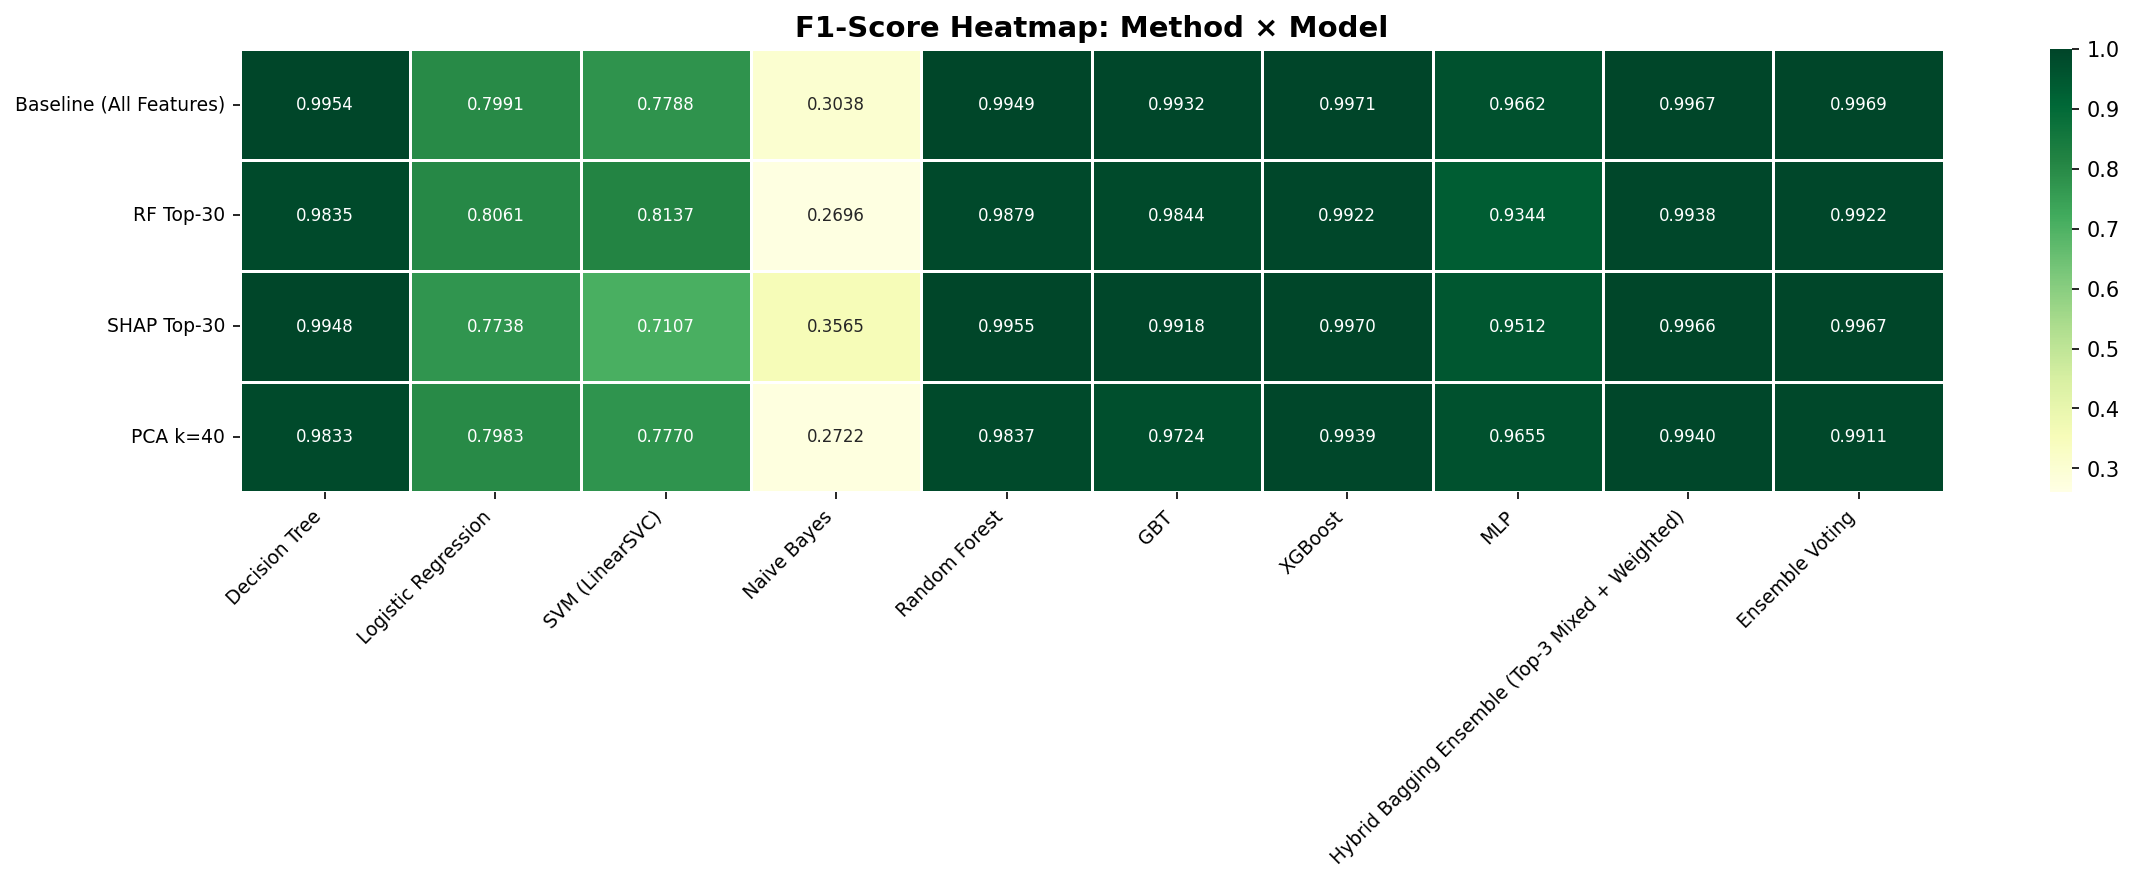
\includegraphics[width=0.62\textwidth]{f1_heatmap.png}%
  }{%
    \fbox{\parbox{0.88\textwidth}{\centering\vspace{1.5cm}\ph{F1 heatmap: method x algorithm --- run papers/fair2026/collect\_results.sh}\vspace{1.5cm}}}%
  }
  \caption{F1 heatmap by method and algorithm (binary, port removed).}
  \label{fig:f1-heatmap}
\end{figure*}

Table~\ref{tab:best-results} summarizes the best model per method, and Figure~\ref{fig:f1-heatmap} visualizes F1 for each method~$\times$~algorithm pair. The comparison design aims to verify whether feature selection (RF/SHAP Top-30) retains near-baseline performance while cutting $\approx$60\% of the features; PCA $k{=}40$ reduces dimensionality in an unsupervised manner at the cost of explainability. All quantitative values are taken directly from the released pipeline outputs.

\begin{table*}[htbp]
  \caption{Summary of the best model per method (values from the released experiment outputs).}
  \label{tab:best-results}
  \centering
  \begin{tabular}{llcccc}
    \toprule
    Method & Model & F1 & AUC-PR & Train (s) & Size (MB) \\
    \midrule
    Baseline & XGBoost & 0.9971 & 0.9999 & 4615.5 & 2.32 \\
    RF Top-30 & XGBoost & 0.9922 & 0.9998 & 1295.1 & 2.52 \\
    SHAP Top-30 & XGBoost & 0.9970 & 0.9999 & 1226.1 & 0.003$^{\dagger}$ \\
    PCA $k$=40 & XGBoost & 0.9939 & 0.9998 & 1444.8 & 3.82 \\
    \bottomrule
  \end{tabular}

  \vspace{2pt}
  {\scriptsize $^{\dagger}$Sizes are obtained by serializing each fitted model \emph{on the training cluster}; the distributed model-saving step writes the tree-ensemble data partitions on whichever executor holds them, so entries in the KB range (here 0.003\,MB) capture only the driver-local metadata and \emph{under-report} the true size. Since the size of a tree ensemble is governed by the number of trees and nodes rather than by the number of input features, the SHAP Top-30 XGBoost model is in reality comparable to its RF Top-30 counterpart ($\approx$2.5\,MB). For the same reason, a reduced feature set can even yield a slightly \emph{larger} model than the baseline (2.52 vs.\ 2.32\,MB): with fewer split candidates the trees need more nodes to reach comparable purity. The single-node export of the deployed pipeline measures model sizes reliably.}
\end{table*}

\begin{figure}[htbp]
  \centering
  \IfFileExists{../../../results/ml_07_cross_method_comparison/train_predict_time.png}{%
    \includegraphics[width=0.74\columnwidth]{train_predict_time.png}%
  }{%
    \fbox{\parbox{0.9\columnwidth}{\centering\vspace{1.2cm}\ph{Training/prediction time --- run ml\_07\_cross\_method\_comparison.py}\vspace{1.2cm}}}%
  }
  \caption{Training and inference time of each method's representative model on the training Spark cluster (Section~\ref{sec:exp}).}
  \label{fig:timing}
\end{figure}

\subsection{Statistical testing (paired resampling)}

Table~\ref{tab:stat} reports the mean F1 $\pm$ 95\% CI ($t$ distribution) over $N{=}6$ resamplings for the two top methods, together with the paired permutation-test $p$-value. The two methods differ significantly only at the floor of the test's resolution ($p\approx0.031$, Cohen's $d\approx1.94$), yet the absolute F1 gap is about 0.0001. A significance test cannot establish equivalence, so we add two one-sided tests (TOST~\cite{schuirmann1987tost}) against a 0.001 F1 margin fixed in advance, on the Nadeau--Bengio error: $p_{\text{TOST}}=3.9\times10^{-6}$, the tightest margin these six splits support at $\alpha=0.05$ being $\pm2.3\times10^{-4}$ F1 --- equivalence in the positive sense, not mere indistinguishability.

\begin{table}[htbp]
  \caption{Multi-resampling stability and paired testing (values from the released experiment outputs).}
  \label{tab:stat}
  \centering
  \footnotesize
  \begin{tabular}{llcc}
    \toprule
    Method & Model & F1 (mean $\pm$ CI95) & $p$ (paired) \\
    \midrule
    Baseline & XGBoost & 0.99734 $\pm$ 0.00007 & \multirow{2}{*}{0.031} \\
    SHAP Top-30 & XGBoost & 0.99720 $\pm$ 0.00009 & \\
    \bottomrule
  \end{tabular}
\end{table}

\subsection{Robustness and multiclass evaluation}

In the in-distribution stability check (a subset of the test set), the ranking of the methods is preserved (XGBoost leads in all four methods). The multiclass evaluation (Figure~\ref{fig:cm}, Table~\ref{tab:perclass}) shows a wide gap between weighted-F1 ($\approx$0.998) and macro-F1 ($\approx$0.806): the rare classes carry the loss. Reading the confusion matrix by where the errors land separates two failure modes. XSS is mostly mislabeled but still detected: 81/111 samples are predicted as Web Brute Force, so at the binary (deployment) level 76\% of XSS flows are still flagged as attacks. The damaging mode is leakage into Benign: all 6 SQL Injection samples, 54\% of Bot (158/290), and 27\% of Web Brute Force are predicted benign. Three mechanisms drive this: extreme imbalance (6--311 samples vs.\ 380k benign); removing \texttt{destination\_port} hits web attacks hardest, since without the port-80 shortcut their short HTTP flows resemble ordinary browsing, so the 0.027 recall here replaces a leakage-inflated one; and Bot C\&C beaconing resembles background traffic once service identity is gone. Targeted imbalance handling and temporal features for beaconing follow as future work.

\begin{figure}[htbp]
  \centering
  \IfFileExists{../../../results/ml_09_multiclass_eval/confusion_matrix.png}{%
    
\includegraphics[width=0.64\columnwidth]{confusion_matrix.png}%
  }{%
    \fbox{\parbox{0.9\columnwidth}{\centering\vspace{1.2cm}\ph{Multiclass confusion matrix --- run ml\_09\_multiclass\_eval.py}\vspace{1.2cm}}}%
  }
  \caption{Multiclass confusion matrix (row-normalized).}
  \label{fig:cm}
\end{figure}

\begin{table}[htbp]
  \caption{Per-class Precision/Recall/F1 (from the released experiment outputs).}
  \label{tab:perclass}
  \centering
  \resizebox{\columnwidth}{!}{%
  \begin{tabular}{lcccc}
    \toprule
    Class & Support & Precision & Recall & F1 \\
    \midrule
    Benign & 380,119 & 0.9981 & 0.9997 & 0.9989 \\
    DoS Hulk & 34,446 & 0.9990 & 0.9904 & 0.9947 \\
    PortScan & 383 & 1.0000 & 0.9530 & 0.9759 \\
    Web Attack~-- Brute Force & 311 & 0.7346 & 0.7299 & 0.7323 \\
    Bot & 290 & 1.0000 & 0.4552 & 0.6256 \\
    Web Attack~-- XSS & 111 & 1.0000 & 0.0270 & 0.0526 \\
    Infiltration & 12 & 1.0000 & 0.6667 & 0.8000 \\
    Web Attack~-- SQL Injection & 6 & 0.0000 & 0.0000 & 0.0000 \\
    \multicolumn{5}{c}{\footnotesize 7 remaining classes, all F1 $\geq 0.95$; see released outputs} \\
    \multicolumn{5}{c}{\footnotesize macro-F1 $=0.806$ \quad weighted-F1 $=0.998$} \\
    \bottomrule
  \end{tabular}}
\end{table}

\subsection{Cross-dataset generalization}
\label{sec:cross-dataset}

To go beyond \emph{in-domain} evaluation, we train on one dataset and test on the other (cross-dataset evaluation, run in both directions) on the leakage-free feature set shared by the two datasets. Because CSE-CIC-IDS2018~\cite{csecicids2018} is very large ($\sim$16M flows) we use a label-stratified sample (fraction 0.2, fixed seed): $\sim$3.14M flows, $\sim$2.39M after feature-level deduplication, against $\sim$2.23M for CICIDS2017.

\begin{table}[htbp]
  \caption{Cross-dataset generalization (2017 = CICIDS2017, 2018 = CSE-CIC-IDS2018):
  mean of four runs differing only in the forest seed; 95\% interval on cross-dataset F1.}
  \label{tab:cross-dataset}
  \centering
  \footnotesize
  \begin{tabular}{lcc}
    \toprule
    Train $\to$ Test & F1 & AUC-PR \\
    \midrule
    2017 $\to$ 2017 (in-domain) & 0.9954 & 0.9997 \\
    2017 $\to$ 2018 (cross) & 0.2154 $\pm$ 0.2562 & 0.4989 \\
    2018 $\to$ 2018 (in-domain) & 0.9243 & 0.9675 \\
    2018 $\to$ 2017 (cross) & 0.0536 $\pm$ 0.0116 & 0.1862 \\
    \bottomrule
  \end{tabular}
\end{table}

The contrast is the sharpest result in the paper: in-domain F1 is high and stable in both directions (0.9954 and 0.9243, CV $<$0.1\%), yet cross-dataset performance collapses --- most clearly in the threshold-free AUC-PR, 0.9997 to 0.4989 and 0.9675 to 0.1862. Cross-dataset F1 averages 0.2154 and 0.0536 at very low recall (0.126 and 0.030) but still-usable precision (0.850 and 0.248): the model misses the other testbed's attacks rather than alarming indiscriminately. That F1 is also irreproducible: four identical runs span 0.0449--0.3009 for 2017$\to$2018, and two runs sharing a seed disagree. At such low recall nearly every target attack flow sits just below the 0.5 threshold, so split points shifted by floating-point aggregation order flip a whole cluster of near-identical flows at once, while AUC-PR varies by 6\% where F1 varies by 55\%. We therefore average F1 over runs and judge the gap on AUC-PR. The causes are concrete: a different CICFlowMeter version (changed feature scales), a different network configuration, and non-overlapping attack tooling (HOIC/LOIC-HTTP exist only in 2018). Is it merely a scale mismatch? Two classic unsupervised adaptations --- refitting the scaler on the target, and CORAL~\cite{sun2016coral}, both without target labels or retraining --- recover no F1 (0.000 either direction), so the shift sits in the conditional distribution, not the first two moments. CORAL does lift AUC-PR for 2018$\to$2017 (0.199 to 0.258) with F1 still zero: the ranking improves, the source-fitted 0.5 threshold does not survive, and adaptation here has to recalibrate the threshold as well as the features. Labelling a little of the new network works immediately: retraining on 1\% of the target's training split (19k flows) reaches F1 0.92 and 0.99, and pooling them with the 1.79M source flows is worse (0.80, 0.96) than dropping the source data. The new network is not hard to detect on; the old model is what fails to transfer. This collapse is consistent with prior cross-dataset IDS studies~\cite{dhooge2020interdataset,cantone2024crossdataset} and reinforces the central claim of this paper: near-perfect in-domain scores (even leakage-free ones) do not certify deployability under distribution shift, so cross-dataset evaluation must be a mandatory part of IDS validation, and domain adaptation is a prerequisite for practical transfer.

\section{Discussion}
\label{sec:discuss}

\textbf{Method comparison.} Baseline and SHAP Top-30 are equivalent within $\pm2.3\times10^{-4}$ F1 (Table~\ref{tab:stat}), so secondary criteria --- explainability, size, stability, feature count --- decide the deployment choice. RF Top-30 trails SHAP Top-30 by $\approx$0.005 F1 at the same feature count, and SHAP Top-30 also yields consistent local explanations for SOC operations.

\textbf{Bridge to the edge device.} Cutting $\approx$60\% of the features reduces vector-assembly cost and model footprint on the Jetson Orin Nano Super, so the selection criterion has to weigh feature count, model size and training/prediction time (Figure~\ref{fig:timing}) alongside F1. Latency and throughput on the Jetson appear in a companion systems paper.

\textbf{Limitations of the binary evaluation.} Removing the port and deduplicating brings binary F1 down to a realistic level, but binary classification remains a relatively easy task. Only under multiclass evaluation do the weaknesses on rare attack classes emerge, and this is also a more reliable metric for distinguishing methods.

\section{Threats to Validity}
\label{sec:threats}

\textbf{Internal validity.} The RF/SHAP rankings are derived from the original training set and kept fixed across resamplings, which follows the ``a priori configuration'' design but lets the ranking see flows that a later resampling puts in its test split. Re-ranking SHAP inside a resampling is expensive, so we did it for two of the six: F1 moved by at most $7.4\times10^{-5}$, in opposite directions, and 25--26 of the 30 features were reselected. The fixed ranking is not inflating F1. The Top-3 component models of the ensemble are selected on that same held-out validation set, at the cost of training the base models on less data. Class balancing applies to all models except MLP (Spark ML offers no sample weights for it), so the MLP result carries that caveat.

\textbf{External validity.} CICIDS2017 (2017) may not reflect current traffic, and benchmark NIDS datasets carry documented quality limitations~\cite{goldschmidt2025datasets}; verification on newer datasets (CSE-CIC-IDS2018, CIC-IoT) is needed. The default random split shuffles time; a time-based split is also supported. The cross-dataset conclusion (Section~\ref{sec:cross-dataset}) rests on a stratified sample of CSE-CIC-IDS2018, not the whole set. The model assumes an attack distribution approximating CICIDS2017 and has not been tested against deliberately evasive traffic, and feature-level deduplication itself shifts the benign/attack ratio.

\textbf{Statistical validity.} Cross-dataset F1 is not deterministic across runs (Section~\ref{sec:cross-dataset}), so it is reported as a mean over $n{=}4$ runs and each adaptation figure is compared within its own run. The small sample size ($N{=}6$) gives the equivalence test low power: because the permutation test is two-sided, the smallest attainable $p$ is only $2/2^N$, so $N{=}6$ just barely reaches the $0.05$ threshold and can hardly detect small effects. The equivalence claim does not rest on that $p$-value, however: the TOST of Section~\ref{sec:eval} tests it directly, against the same Nadeau--Bengio error that accounts for the overlap between resamplings. Increasing $N$ by nested cross-validation is the next step.

\section{Conclusion}
\label{sec:conclude}

This paper compares four dimensionality-reduction strategies for IDS on Spark ML under a leakage-aware and statistically tested evaluation pipeline. The contribution lies as much in how to evaluate reliably as in which method wins: removing the leaking feature, deterministic feature-level deduplication, model selection on a validation set, exact-enumeration paired testing with Nadeau--Bengio correction, multiclass evaluation, and cross-dataset generalization between CICIDS2017 and CSE-CIC-IDS2018 (Section~\ref{sec:cross-dataset}). Future directions: an ablation of the deduplication step itself, the second leakage source; the full CSE-CIC-IDS2018 and newer datasets (RoEduNet, CIC-IoT); transferability of the SHAP Top-30 set between datasets; and real-time edge deployment.

\section*{Acknowledgment}
The authors declare no conflict of interest.

{\footnotesize
\setlength{\IEEEbibitemsep}{0pt}
\bibliographystyle{ieeetr}
\bibliography{references,../../latex/related_work}}

\end{document}
